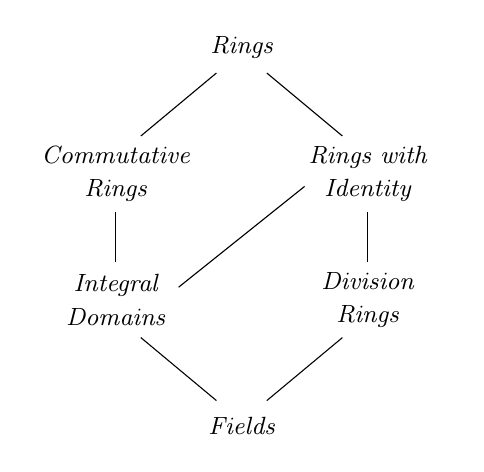
\begin{tikzpicture}[scale=0.8]

\draw  (2,0.4) -- (2,-0.4);
\draw  (-2,0.4) -- (-2,-0.4);
\draw  (1,0.8) -- (-1,-0.8);
\draw  (1.6,1.6) -- (0.4,2.6);
\draw  (-1.6,1.6) -- (-0.4,2.6);
\draw  (1.6,-1.6) -- (0.4,-2.6);
\draw  (-1.6,-1.6) -- (-0.4,-2.6);

\node [text width=2cm, text centered] at (2, 1) {\small \it Rings with Identity};
\node [text width=1.5cm, text centered] at (2, -1) {\small \it Division Rings};

\node [text width=2cm, text centered] at (-2, 1) {\small \it Commutative Rings};
\node [text width=1.5cm, text centered] at (-2, -1) {\small \it Integral Domains};

\node at (0,3) {\small \it Rings};
\node at (0,-3) {\small \it Fields};
\end{tikzpicture}
